\apendice{Manual de especificación del diseño}
En este trabajo se ha realizado la implementación de diferentes modelos epidemiológicos deterministas utilizando diversas herramientas del entorno de MATLAB.
\section{Diagramas de bloques}
Se han utilizado diagramas de bloques en \textbf{Simulink} para representar los distintos modelos epidemiológicos (SI, SIS, SIR, SEIR, SIRV y SEIRV). 
Estos diagramas no constituyen planos técnicos tradicionales, pero permiten visualizar de forma clara y esquemática la estructura dinámica de cada modelo, mostrando las interacciones entre los compartimentos y facilitando la comprensión y simulación del sistema.

A continuación se muestran los diagramas de bloques para cada modelo.

\textbf{Modelo SI} representado en la figura \ref{fig: diagrama de bloques en Simulink para el modelo SI}, representa la dinámica básica entre individuos susceptibles e infectados, asumiendo que una vez infectados, permanecen en ese estado sin recuperación.
\begin{figure}[H]
        \centering
        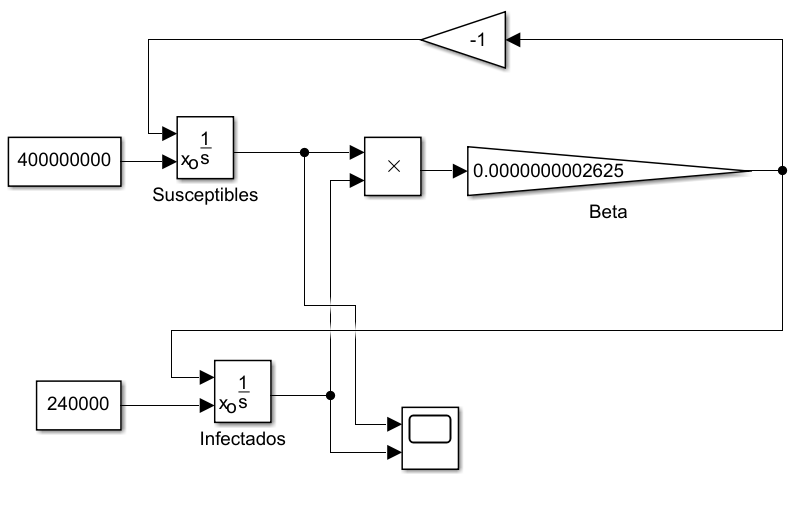
\includegraphics[width=0.9\textwidth]{img/modelo_SI.png}
        \caption{Diagrama de bloques en Simulink para el modelo SI.}
        \label{fig: diagrama de bloques en Simulink para el modelo SI}
        
\end{figure}

\textbf{Modelo SIS} representado en la figura \ref{fig: diagrama de bloques en Simulink para el modelo SIS}, contempla que los individuos infectados pueden recuperarse pero sin adquirir inmunidad, volviendo al estado susceptible.
\begin{figure}[H]
        \centering
        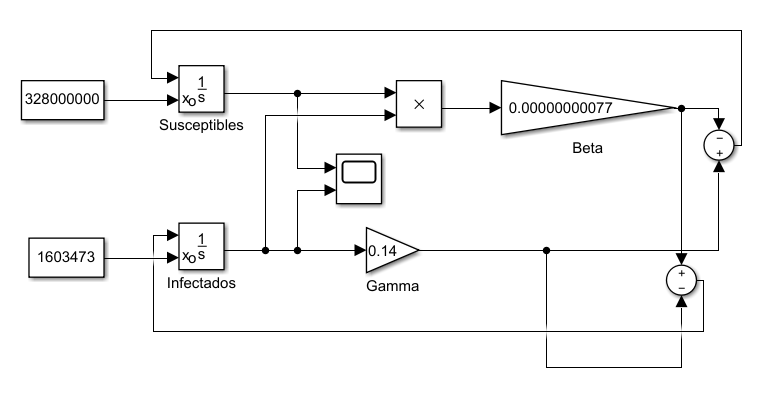
\includegraphics[width=0.9\textwidth]{img/modelo_SIS.png}
        \caption{Diagrama de bloques en Simulink para el modelo SIS.}
        \label{fig: diagrama de bloques en Simulink para el modelo SIS}
        
\end{figure}

\textbf{Modelo SIR} representado en la figura \ref{fig: diagrama de bloques en Simulink para el modelo SIR}, los individuos susceptibles pueden infectarse, pasar a infectados y posteriormente recuperarse con inmunidad permanente.


\begin{figure}[H]
        \centering
        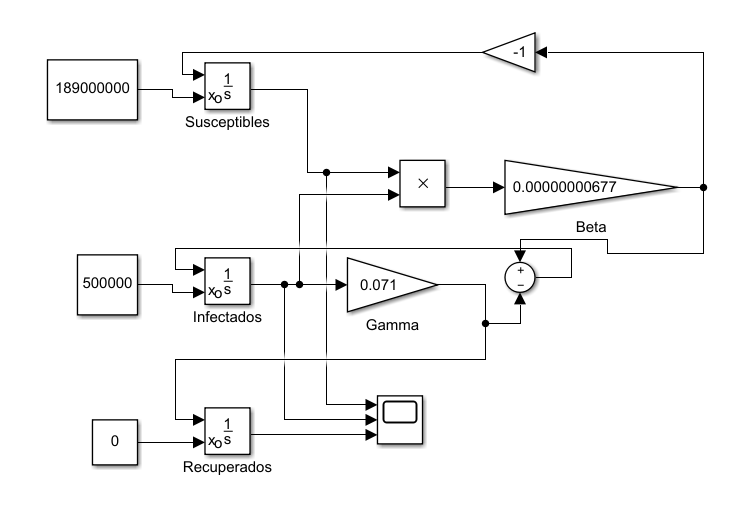
\includegraphics[width=0.9\textwidth]{img/modelo_SIR.png}
        \caption{Diagrama de bloques en Simulink para el modelo SIR.}
        \label{fig: diagrama de bloques en Simulink para el modelo SIR}
        
\end{figure}


\textbf{Modelo SIR con regulador PID} representado en la figura \ref{fig: diagrama de bloques en Simulink para el modelo SIR con regulador PID} corresponde a una extensión del modelo SIR clásico en la que se incorpora un controlador PID. Este regulador actúa sobre la tasa de transmisión con el objetivo de mantener la proporción de individuos infectados por debajo de un valor de referencia, simulando medidas de control sanitario como confinamientos, campañas de vacunación o restricciones de movilidad. El sistema ajusta dinámicamente la intensidad de dichas medidas en función del error entre el número de infectados reales y el deseado, permitiendo evaluar la efectividad de estrategias de intervención automática en la evolución de la epidemia.
\begin{figure}[H]
        \centering
        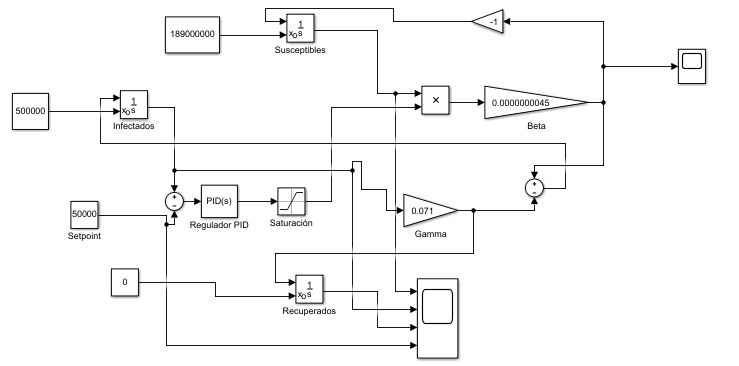
\includegraphics[width=0.9\textwidth]{img/modelo SIR con PID.png}
        \caption{Diagrama de bloques en Simulink para el modelo SIR con regulador PID.}
        \label{fig: diagrama de bloques en Simulink para el modelo SIR con regulador PID}
        
\end{figure}



\textbf{Modelo SEIR} representado en la figura \ref{fig: diagrama de bloques en Simulink para el modelo SEIR}, extensión del modelo SIR que incluye una fase de exposición, donde los individuos están infectados pero no son contagiosos durante un período de incubación.
\begin{figure}[H]
        \centering
        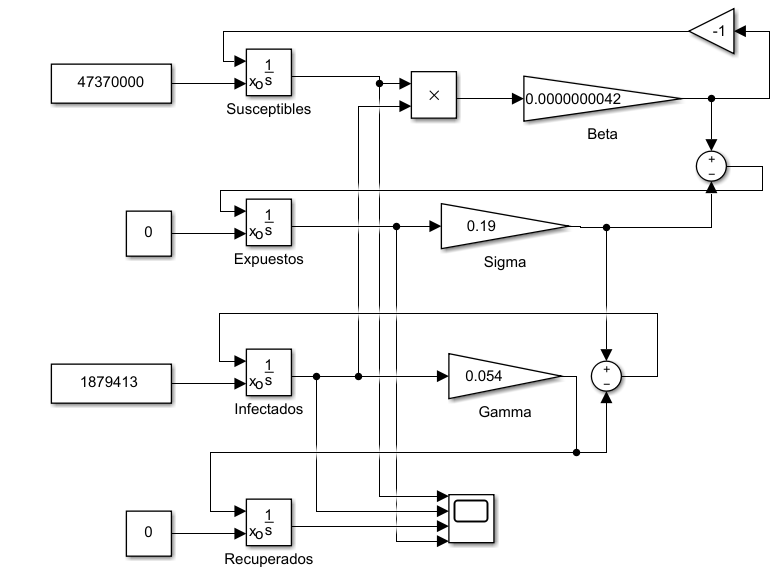
\includegraphics[width=0.9\textwidth]{img/modelo_SEIR.png}
        \caption{Diagrama de bloques en Simulink para el modelo SEIR.}
        \label{fig: diagrama de bloques en Simulink para el modelo SEIR}
        
\end{figure}

\textbf{Modelo SIRV} representado en la figura \ref{fig: diagrama de bloques en Simulink para el modelo SIRV}, modelo SIR que incorpora la vacunación como una vía adicional para pasar de susceptibles a inmunes sin pasar por la infección.
\begin{figure}[H]
        \centering
        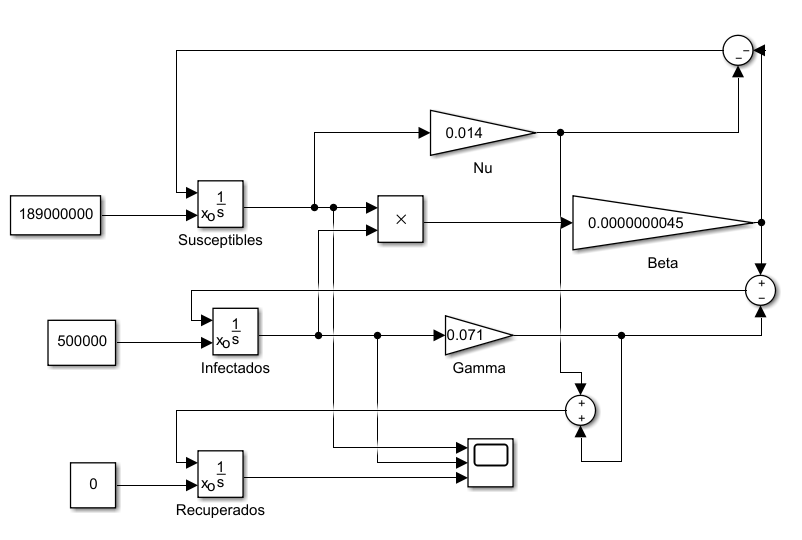
\includegraphics[width=0.9\textwidth]{img/modelo_SIRV_inicio.png}
        \caption{Diagrama de bloques en Simulink para el modelo SIRV.}
        \label{fig: diagrama de bloques en Simulink para el modelo SIRV}
        
\end{figure}


\textbf{Modelo SEIRV} representado en la figura \ref{fig: diagrama de bloques en Simulink para el modelo SEIRV}, modelo SEIR que añade un compartimento para vacunados, permitiendo estudiar el impacto de la vacunación en la dinámica de la epidemia.
\begin{figure}[H]
        \centering
        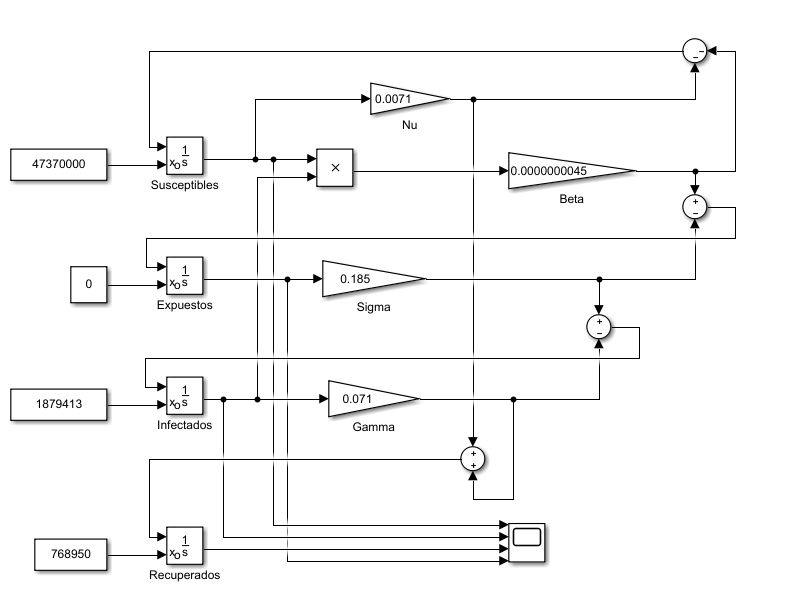
\includegraphics[width=0.9\textwidth]{img/modelo_SEIRV.png}
        \caption{Diagrama de bloques en Simulink para el modelo SEIRV.}
        \label{fig: diagrama de bloques en Simulink para el modelo SEIRV}
       
\end{figure}


\section{Diseño arquitectónico}
El sistema desarrollado consta de tres componentes principales:

\begin{itemize}
    \item \textbf{Modelos en Simulink:} cada modelo epidemiológico se implementa mediante diagramas de bloques que representan las ecuaciones diferenciales del sistema. Esto permite simular la dinámica de la epidemia de manera visual e intuitiva.

    \item \textbf{Scripts en MATLAB:} se utiliza para la implementación del controlador PID en el modelo SIR, actuando sobre la tasa de transmisión para mitigar la propagación.

    \item \textbf{Interfaz gráfica en App Designer:} diseñada para permitir al usuario modificar parámetros epidemiológicos y del controlador, ejecutar simulaciones y visualizar resultados de forma interactiva mediante gráficas dinámicas.
\end{itemize}



En cunato a la aplicación ha sido desarrollada en MATLAB App Designer, lo que proporciona una arquitectura de programación basada en eventos y de programación declarativa para la interfaz de usuario, donde la interfaz gráfica y la lógica de control están encapsuladas en un único archivo `.mlapp'.

El diseño se estructura en los siguientes componentes principales:

\begin{itemize}
    \item \textbf{Interfaz de usuario (UI):} compuesta por elementos gráficos como botones, menús desplegables, campos de entrada numérica y ejes para visualización. Permite al usuario seleccionar el modelo epidemiológico, definir los parámetros iniciales, ejecutar la simulación y visualizar los resultados.
    
    \item \textbf{Controladores (callbacks):} funciones asociadas a eventos de la interfaz gráfica, tales como la selección del modelo o la pulsación del botón de simulación. Estas gestionan la lógica de interacción entre la UI y el núcleo del programa.
    
    \item \textbf{Módulo de simulación:} implementado mediante funciones anónimas de MATLAB y el solucionador \texttt{ode45}, permite resolver los distintos modelos epidemiológicos (SI, SIS, SIR, SEIR, SIRV, SEIRV) a partir de los parámetros definidos por el usuario.
    
    \item \textbf{Visualización de resultados:} Utiliza la función \texttt{plot} para representar la evolución temporal de las variables del modelo. Las leyendas y los ejes se ajustan dinámicamente según el modelo seleccionado.
\end{itemize}


\textbf{Diagrama de clases}.
La clase principal aplicacion\_modelos agrupa todos los elementos de la interfaz de usuario (UI), así como las funciones necesarias para gestionar eventos y simular los modelos epidemiológicos. Se emplea un enfoque orientado a eventos, donde la lógica de simulación se encuentra encapsulada en funciones de devolución de llamada (callbacks). El diagrama de clases se puede ver en la figura \ref{fig: diagrama de clases de la aplicación realizada.}.

\begin{figure}[H]
        \centering
        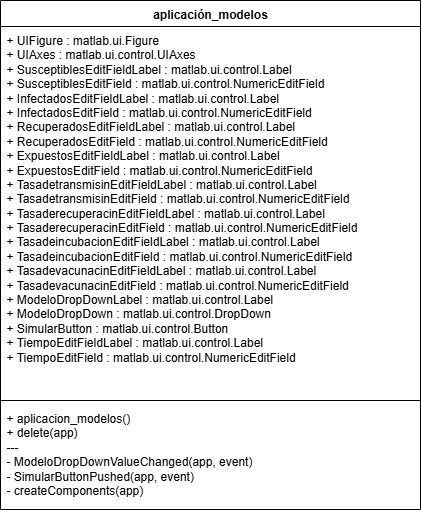
\includegraphics[width=0.9\textwidth]{img/Diagrama sin título.drawio.png}
        \caption{Diagrama de clases de la aplicación realizada.}
        \label{fig: diagrama de clases de la aplicación realizada.}   
\end{figure}








